\documentclass{standalone}

\usepackage{xcolor}
\definecolor{linkcolor}{RGB}{168, 141, 201}

\usepackage{tikz}
\usetikzlibrary{arrows.meta, arrows, backgrounds, bayesnet, calc, matrix}

\begin{document}

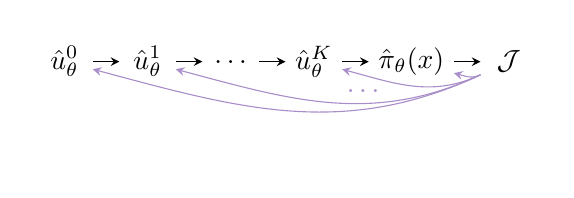
\begin{tikzpicture}
  \matrix (m) [
      matrix of math nodes,row sep=2em,column sep=1em,
      minimum width=2em,nodes={anchor=center}
  ] {
    \hat u^{0}_\theta & \hat u_\theta^{1} &
    \ldots & \hat u_\theta^{K} & \hat \pi_\theta(x) & \mathcal{J} \\
    \; & \; & \; & \; & \; & \; \\};
  \node at (1.,0.1) () {\color{linkcolor}\ldots};
  \path[-stealth]
    (m-1-1) edge node {} (m-1-2)
    (m-1-2) edge node {} (m-1-3)
    (m-1-3) edge node {} (m-1-4)
    (m-1-4) edge node {} (m-1-5)
    (m-1-5) edge node {} (m-1-6)
    (m-1-6) edge[draw=linkcolor,out=-155,in=-15] node[below] {} (m-1-5)
    (m-1-6) edge[draw=linkcolor,out=-155,in=-15] node {} (m-1-4)
    (m-1-6) edge[draw=linkcolor,out=-155,in=-15] node {} (m-1-2)
    (m-1-6) edge[draw=linkcolor,out=-155,in=-15] node {} (m-1-1)
    ;
\end{tikzpicture}
\end{document}